\subsubsection{Context}

Conventional systems neuroscience experiments are typically short in duration
and often place significant constraints on subjects behaviours to simplify data
analysis.
%
However, these restrictions may limit our ability to observe critical
aspects of brain function and behaviour that only manifest in more naturalistic
and extended conditions.

At the Sainsbury Wellcome Centre (SWC) and Gatsby Computational Neuroscience
Unit (GCNU) we are pioneering \textbf{Naturalistic, Long-Duration, and
Continual (NaLoDuCo) experiments} in mice that span weeks to months. During
these experiments, we collect high-resolution behavioural and neural recordings
in naturalistic settings (Figure~\ref{fig:aeon}).

\begin{figure}
    \begin{center}
        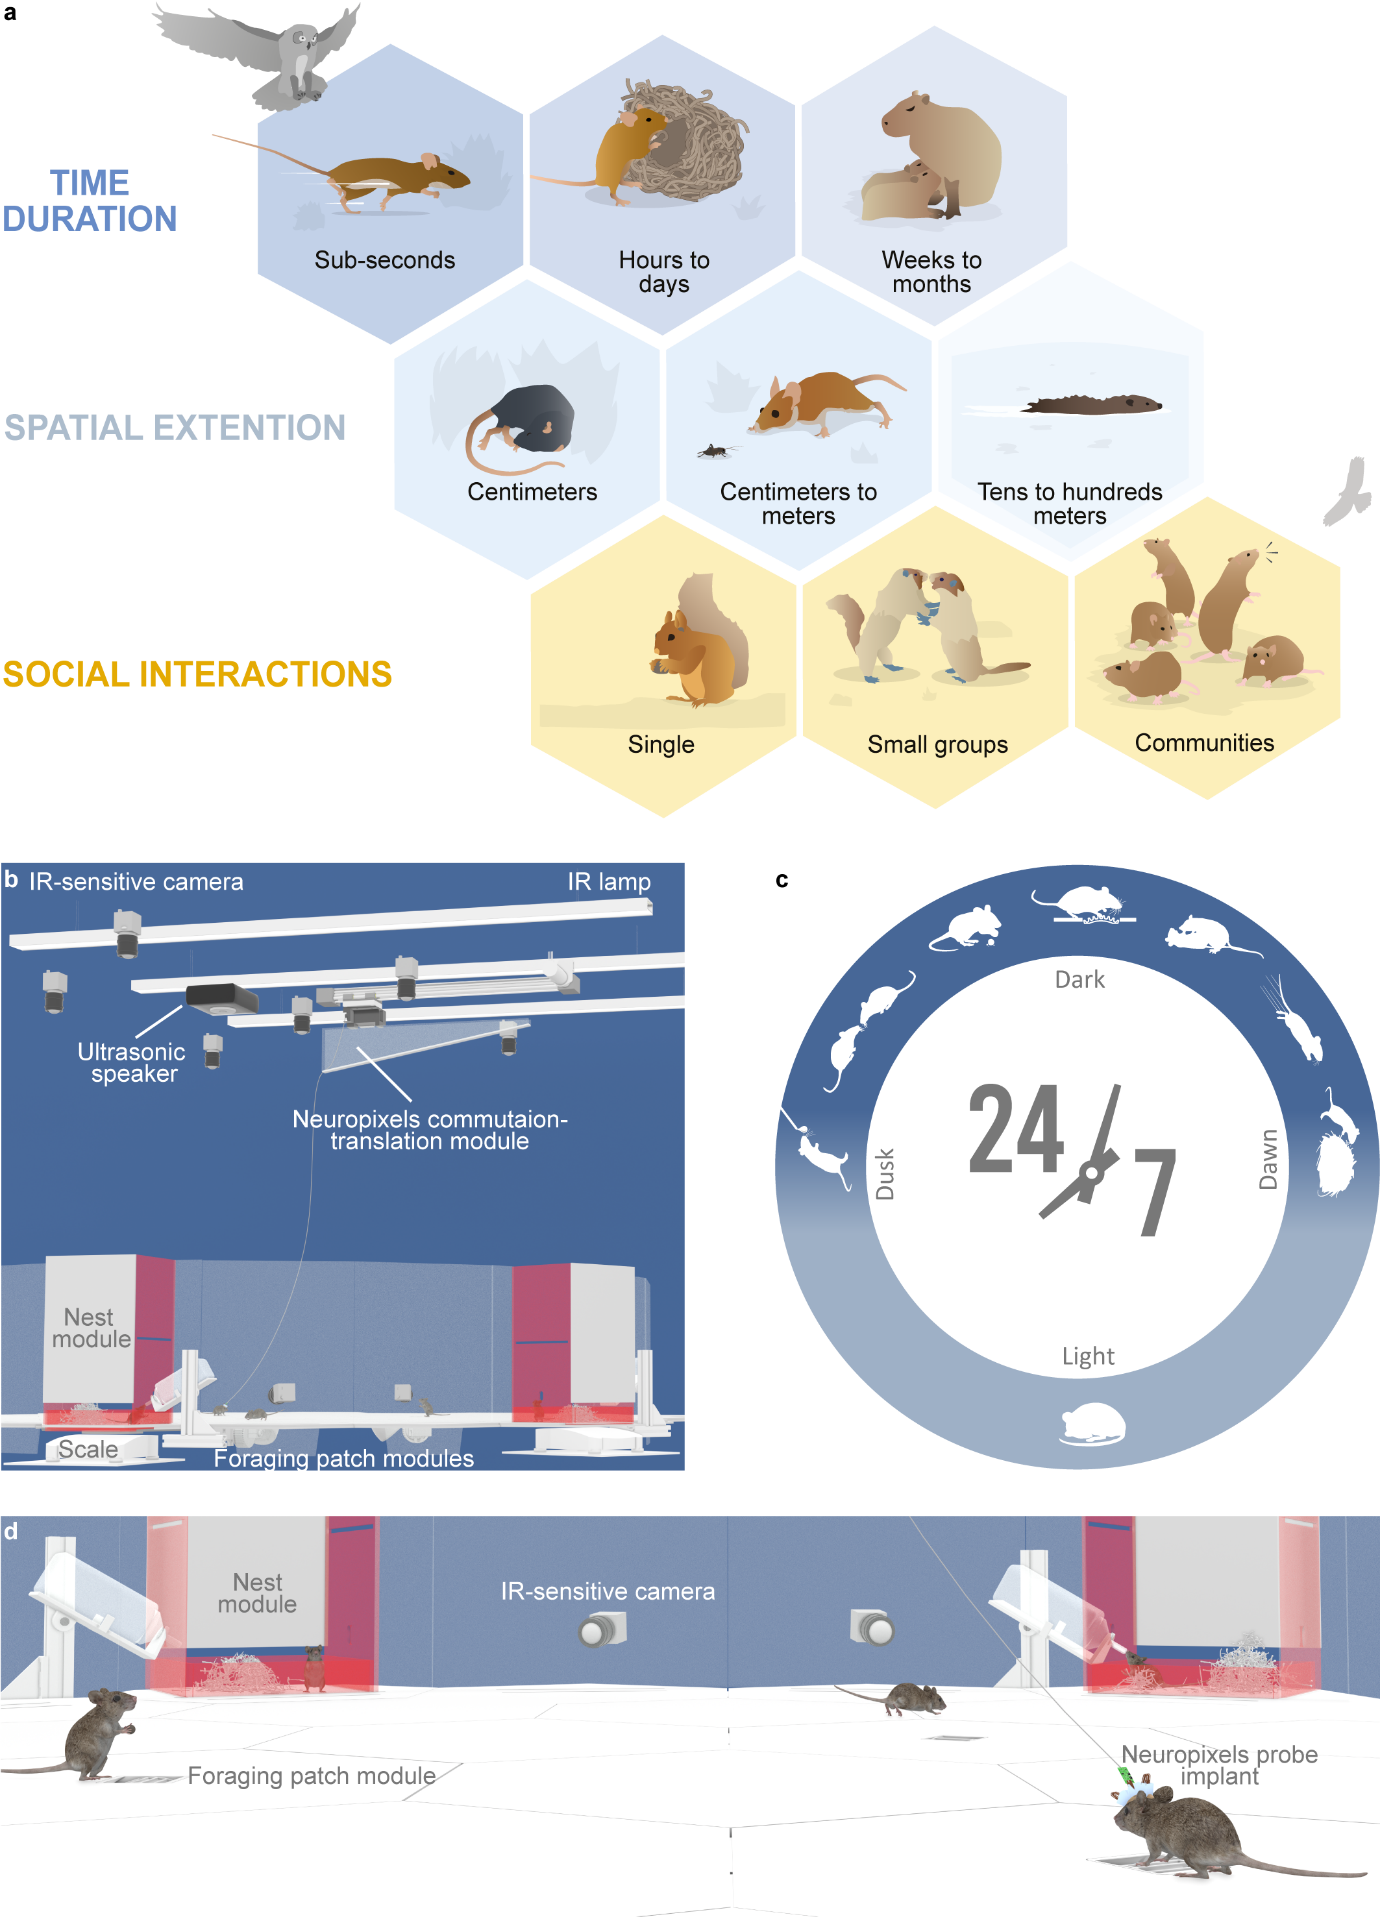
\includegraphics[width=4in]{figures/aeon.png}
    \end{center}
    \caption{\textbf{a}: Example of natural behaviours in rodents that take place over
    different timescale, spatial extensions and involving different numbers of
    individuals.\\
    \textbf{b-d}: Close-up views of one possible configuration of the Aeon environment
    in which naïve mice and mice chronically implanted with Neuropixels probe
    can live while expressing a variety of natural behaviours including
    exploring, drinking, escaping, foraging, nesting, sleeping, eating and
    interacting socially.}
    \label{fig:aeon}
\end{figure}

To support this endeavour, we are developing the \textbf{AEON platform}, an
innovative set of hardware and software tools for NaLoDuCo experimental
control, data store and access. We are using this platform to investigate the
neural basis of foraging behaviour in mice over prolonged periods of
time~\citep{campagnerEtAl24}.

Our US partner, the \textbf{Allen Institute for Neural Dynamics (AIND)} is also
performing NaLoDuCo experimentation, using the AEON platform, studying
naturalistic olfactory learning over weeks to month outside conventional task
structures~\citep{finkEtAl24}.

\textbf{NeuroGEARS Ltd}, our industrial partner, is a UK-based company
supporting academic institutions implementing innovative technology for
scientific investigation.
%
It is the main developer of the \textbf{Bonsai} software ecosystem for
experimental control~\citep{lopesEtAl15}, used by thousands of scientists
around the world, and powering the AEON platform.
%
NeuroGEARS  has played a central role in the development of the AEON platform,
and provides services to both the SWC and the AIND.

NaLoDuCo experimentation will enable researchers to explore neural mechanisms
underlying ethological behaviours in naturalistic environments over months, for
the first time.  The experiments will shed new light on a wide range of poorly
understood neural mechanisms, including how the brain structures complex
behavioural sequences as a function of the animal needs, learning, adaptation,
sleep-dependent memory consolidation and social dynamics.
%
\textbf{The data generated from NaLoDuCo experiments represent an entirely new
resource in neuroscience}, with the potential to drive breakthroughs and
discoveries that are beyond the reach of traditional experiments.

% Since the project started in 2021, our UK business partner, NeuroGEARS Ltd.\
% has been contracted by the SWC to lead the implementation of the NaLoDuCo
% experimental framework. NeuroGEARS also provides services to the AIND.

While \textbf{naturalistic, long-duration, or continuous} neuroscience experiments have
been conducted in the past
\citep{nagyEtAl23,hoEtAl23,rayEtAl25,weissbrodEtAl13,dhawaleEtAl17,newmanEtAl24}, to the
best of our knowledge, \textbf{we are the first ones to integrate all three of these
features in a single experimental paradigm}.
%
% Experiments of this type have been advocated by experts in the field years ago
% \citep[][p19]{dattaEtAl19}, yet they have not been implemented so far.

This emerging paradigm of long-duration experimentation is poised to become
mainstream in the coming years.
%
However, experiments spanning weeks to months generate massive datasets—often
reaching hundreds of terabytes—posing significant challenges in data
acquisition, management, distribution, visualisation, and analysis.
%
To address these challenges, we (GCNU, SWC, AIND, and NeuroGEARS Ltd) will
collaboratively extend the AEON platform with functionality to
\textbf{visualise and statistically analyse previously collected NaLoDuCo
experimental data on the cloud}, and to \textbf{perform real-time machine to enable the
intelligent control of NaLoDuCo experiments}.

\subsubsection{Specific aims}

Data generated by NaLoDuCo experiments will be of general interest to the
neuroscience community. \textbf{We want to share our NaLoDuCo foraging and odour
learning recordings and allow other groups collecting this type of data to
share their own.}
%
However, this dissemination is not trivial, as datasets are of the order of
hundreds of terabytes, and it will take users several days to download them
over standard Internet connections.

Instead of bringing data to users, we will bring users to data, by storing
datasets in the cloud (or in institutional clusters), and providing
\textbf{cloud software to allow users to visually explore and statistically
analyse behavioural and neural NaLoDuCo datasets where they live}
(1 and 2 in Figure~\ref{fig:aims}).

Our statistical analysis of neural time series will require knowledge of the
spiking activity of single units; i.e., spike sorting. In long-duration
experiments with freely moving animals spike sorting is a challenging problem,
because movements of recording probes change the shape of spike waveforms over
time and complicate the assignment of spikes to units based on their waveforms.
We will address this problem by developing \textbf{spike sorting methods for
long-duration, continual and high-channel-count recordings} (3 in
Figure~\ref{fig:aims}).

Funded by a BBSRC award we are adding machine learning functionality to Bonsai
in order to enable a new type of experimentation controlled by advanced machine
learning inference on behavioural and neural
recordings~\citep[Bonsai.ML,][]{bonsaiML25}. We have developed this
functionality for conventional short duration experiments. We will add to
Bonsai.ML \textbf{real-time machine learning functionality for processing
nonstationary data}, such as that generated in NaLoDuCo experiments.

Most of the online neural data analysis methods that we will add to AEON
require sorted spikes. We will adapt the previous offline \textbf{spike sorting
methods for long-duration experiment to operate in real-time} (5 in
Figure~\ref{fig:aims}).

\begin{figure}
    \begin{center}
        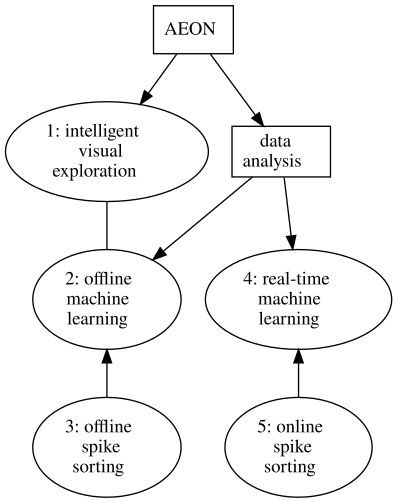
\includegraphics[width=3in]{figures/aims.png}
    \end{center}
    \caption{Specific aims}
    \label{fig:aims}
\end{figure}

